\documentclass{getwriting}
\title{Evaluating infection-generating processes for infectious disease situational awareness: Is the renewal process necessary?}
\author[1]{Samuel P. C. Brand \orcidlink{0000-0003-0645-5367}}
\author[1,2]{Sam Abbott \orcidlink{0000-0001-8057-8037}}

\affil[1]{\footnotesize Center for Forecasting and Outbreak Analytics, Centers for Disease Control and Prevention, United States of America}
\affil[2]{\footnotesize Centre for Mathematical Modelling of Infectious Diseases, London School of Hygiene \& Tropical Medicine, London, United Kingdom}

\begin{document}

\maketitle

\begin{abstract}
Infectious disease surveillance relies on mathematical and statistical models to generate nowcasts, forecasts, and transmission metrics.
A common assumption is that specific infection-generating processes should be paired with particular surveillance measures, leading to debates about using epidemic growth rates versus effective reproduction numbers for situational awareness.

We develop a flexible framework to systematically evaluate how different infection-generating processes perform across multiple epidemiological outcomes, explicitly examining the decoupling between generative processes and target measures. We test models across simulated scenarios with known outcomes, varying generation interval specifications to assess robustness to misspecification.

[Results to be filled in]

This study provides evidence-based recommendations for model selection in public health surveillance, addressing a critical gap in understanding how different modelling approaches perform across various surveillance tasks.
\end{abstract}

\section{Introduction}

Infectious disease surveillance is fundamental to public health decision-making, with mathematical models increasingly deployed to generate nowcasts, forecasts, and transmission intensity measures such as the effective reproduction number and epidemic growth rate. The relationship between infection-generating processes and their target measures is often assumed but rarely examined. Recent literature has focused on comparing epidemic growth rates with effective reproduction numbers for situational awareness, conflating two distinct questions: which measure provides better situational awareness, and which process better models the infection-generating mechanism.

In nowcasting and short-term forecasting, this distinction is more widely recognised. Lison et al. \cite{lison} found that renewal-based generative processes improved nowcasts of effective reproduction numbers, infections, and reported cases. Renewal processes and other mechanistic models are commonly used in forecasting with the assumption that capturing the transmission mechanism improves forecast performance. However, little systematic work has explored this question, and findings from collaborative forecasting hubs remain inconclusive.

We aim to systematically evaluate how infection-generating processes perform across multiple epidemiological outcomes. We develop a generic model framework informed by common practice in situational awareness modelling \cite{abbott2020epinow2, abbott2021epinowcast, scott2021epidemia, Cori2022}, enabling comparison between approaches while maintaining flexibility to capture diverse infection trajectories. Through simulation studies and real-world case studies, we evaluate key infection-generating processes with various latent processes across multiple surveillance tasks. This work contributes to the theoretical understanding of how different generative processes influence model performance and uncertainty quantification for infectious disease dynamics. Our findings provide evidence-based guidance on selecting appropriate model structures for specific public health applications, potentially improving the accuracy of epidemic monitoring, enabling more reliable forecasts for resource allocation, and enhancing overall epidemic response capabilities.

\section{Methods}

In this section, we describe the components of the generic model framework that we use to  Second, we describe the experimental matrix of generative models, along with different time points, forecast horizons, and potential misspecification of the underlying generation interval. Third, we describe the target epidemiological measures of interest in this study and the surveillance task scenarios that we consider. Fourth, we describe the evaluation metric that we use to evaluate each generative model against each target measure. Finally, we outline the implementation details and define the evaluation metrics for this implementation.

\subsection{Generative model framework for epidemiological data}
This section describes the generic model framework we use to define the generative models used in the rest of the analysis

\subsubsection{Transmission intensity measures}

We consider three transmission intensity measures that can be defined from a series of latent infections. Each is also a target for real-time surveillance.

\begin{itemize}
    \item Logarithmic transformation of latent infections $T(t) = \ln I(t)$.
    \item The time-varying growth rate, $T(t) = r(t) = \ln (I(t) / I(t-1))$.
    \item The time-varying reproductive number $T(t) = \mathcal{R}(t) = I(t) / [I \circ g](t)$, where $x\circ y$ is the discrete convolution of vectors $x$ and $y$.
\end{itemize}

The direct transformation between latent infections $I(t)$ and transmission intensity measures such as $\mathcal{R}(t)$ raises a problem, since both processes cannot be defined independently of each other without causing a contradiction. Which process is treated as generative and which is calculated as a transformation of the other?

In our framework, each generative model that we experiment with defines one of these epidemiological processes as being \textit{primary}. The other epidemiological processes are defined as \textit{secondary}. Secondary epidemiological processes are calculated from their definition as conditional on the latent infections generated.

\subsubsection{Generative model as composed model components}

We divide our generative model for epidemiological data into components\cite{bjornstad2022epidemics}, in this case three. These are:
\begin{enumerate}
    \item The \textit{infection-generating process}. This specifies the structure of the dependency of the new latent incidence over time $t$, $I(t)$, on the past incidence $\{I(s),~s < t\}$, and the primary measure of transmission intensity $T(t)$, for example $T(t)=\mathcal{R}(t)$ could be the time-varying reproductive number.
    \item The stochastic \textit{latent process} $Z(t)$ . The latent process drives the stochastic dynamics of the transmission intensity defined in 1. via direct transformation $T(t) = g(Z(t))$. For example $T(t) = \exp(Z(t))$ where $Z(t)$ is a random walk. 
    \item  The \textit{observation model} defines how the trajectory of latent infections $\{I(s),~s \leq t\}$ is transformed into expected epidemiological data counts $Y(t)$ and the link distribution with actual observations $y(t) \sim f(Y(t), \varphi)$ for some sampling distribution $f$ and observation model parameters $\varphi$. For example, $Y(t) = [I \circ D](t)$ for some observation delay probability distribution D and $f$ could be a negative binomial distribution with mean $Y(t)$ and dispersion parameter $\varphi$.

The model components compose to define the full generative model. The model compositions and dependencies are as follows:

    \item The primary transmission intensity $T(t)$ is defined by combining the choice of the infection-generating process [1.] and the latent process [2.] since the choice of the infection-generating process selects the measure of the primary transmission intensity and the latent process $Z(t)$ generates its trajectory.
    \item The latent infections $I(t)$ are defined by combining the choice of the infection-generating process [1.] and the trajectory of the primary transmission intensity $T(t)$ since the choice of infection-generating process defines how $T(t)$ propagates the infection dynamics.
    \item Secondary transmission intensity measures are defined by the choice of infection-generating process [1.] and the trajectory of latent infections $I(t)$ since secondary transmission intensities are direct transformations in $I(t)$, except for the number of reproductions varying in time that also needs the distribution of the generation interval $g$ defined by the choice of infection-generating process.
    \item The expected observations $Y(t)$ are defined by the choice of the observation model [3.] and the trajectory of latent infections
\end{enumerate}

Figure \ref{fig:model_composition} gives a summary of the modelling components and their interactions.
\begin{figure}[h]
  \centering
  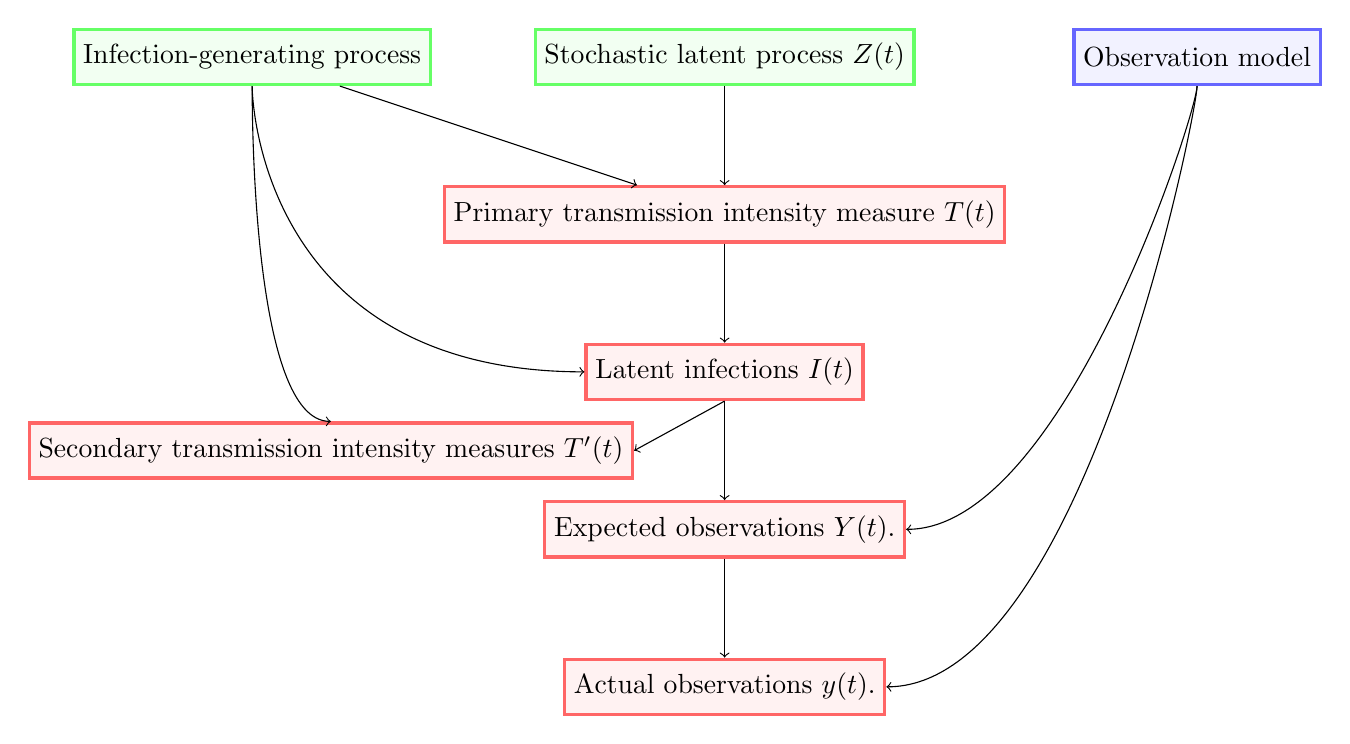
\begin{tikzpicture}[node distance=2cm,
gen_qaunt/.style={draw=red!60, fill=red!5, very thick, minimum size=7mm}, model_spec/.style={draw=green!60, fill=green!5, very thick, minimum size=7mm}, fixed_model_spec/.style={draw=blue!60, fill=blue!5, very thick, minimum size=7mm}]
    % Nodes
    \node (IGP) [draw, model_spec] {Infection-generating process};
    \node (Z) [right of=IGP, xshift=4cm, draw, model_spec] {Stochastic latent process $Z(t)$};
    \node (Obs) [right of=Z, xshift=4cm, draw, fixed_model_spec] {Observation model};
    \node (T) [below of=Z, xshift=0cm, draw, gen_qaunt] {Primary transmission intensity measure $T(t)$};
    \node (I) [below of=T, xshift=0cm, draw, gen_qaunt] {Latent infections $I(t)$};
         \node (T_other) [left of=I, xshift=-3cm, yshift=-1cm,draw, gen_qaunt] {Secondary transmission intensity measures $T'(t)$};
    \node (Y) [below of=I, draw, gen_qaunt] {Expected observations $Y(t)$.};
    \node (yt) [below of=Y, draw, gen_qaunt] {Actual observations $y(t)$.};

    % Arrows
    \draw[->] (IGP) -- node{} (T);
    \draw[->] (Z) -- node{} (T);
    \draw[->] (T) -- node{} (I);
    \draw[->] (IGP) .. controls +(down:7mm) and +(left:4cm) .. (I.west);
    \draw[->] (Obs) .. controls +(down:7mm) and +(right:2cm) .. (Y.east);
    \draw[->] (Obs) .. controls +(down:7mm) and +(right:2.5cm) .. (yt.east);
    % \draw[->] (G.south)  -- node{} (T_other.north);
    % \draw[->] (IGP.south)  -- node{} (T_other.north);
    \draw[->] (IGP) .. controls +(down:7mm) and +(left:1cm) .. (T_other.north);
    \draw[->] (I.south) -- node{} (T_other.east);
    \draw[->] (I) -- node{} (Y);
    \draw[->] (Y) -- node{} (yt);
    
  \end{tikzpicture}
  \caption{Directed graph representing the generative model components. Shown are model choices we experiment over in this study (green rectangles), the observation model (which is fixed in this study; blue rectangle), and generated quantities (red boxes). The generated quantities are split between a primary transmission intensity measure $T(t)$ which composes with the infection-generating process to generate latent infections, and secondary transmission intensity measures.  All transmission intensity measures are targets for surveillance. Each modelled quantity can be constructed conditional on parent quantities on the graph (directed edges).  }
  \label{fig:model_composition}
\end{figure}



\subsection{Latent infection-generating processes}
We consider stochastic process models that can be used to generate infections that won't be directly observed, we call these stochastic process models \textit{latent infection-generating processes}. We further limit our analysis to latent infection-generating processes that can be formulated as a function of a basic noise process $(\epsilon_t)_{t\geq 1}$ where each is independent and identically distributed $\epsilon_t \sim \text{Normal}(0,1)$. This is a discrete-time analogue formulation to using the Wiener process in the construction of stochastic differential models \cite{oksendal2013stochastic}, and therefore, covers a wide range of useful modelling frameworks. 

In epidemiological modelling, it is common to be interested in quantities that summarise the trajectory of underlying infections, for example, the reproductive number \cite{anderson1991infectious,diekmann1990definition,keeling2011modeling} or exponential growth rate \cite{anderson1991infectious,keeling2011modeling} which may themselves be time-varying \cite{gostic2020practical}. It is common for the infection-generating process to be defined in terms of a time-varying reproductive number, for example, the renewal model of latent infections \cite{mishra_derivation_2020} which is the default infection-generating process in several software packages \cite{abbott2020epinow2,scott2021epidemia, Cori2022}. For this reason, we will consider a taxonomy of infection-generating processes which distinguishes between two factors: 
\begin{itemize}
    \item A generating process $(Z_t)_{t\geq 1}$ which has a functional dependence $f_Z$ at each time step $t$ on:
    \begin{itemize}
        \item The noise process up to time $t$, $\epsilon_{t},\epsilon_{t-1},\epsilon_{t-2},\dots$.
        \item Past $Z_{t-1},Z_{t-2},\dots$.
        \item Model parameters $\theta$.
    \end{itemize}
    \item The incidence process $(I_t)_{t\geq 1}$ which has a functional dependence $f_I$ at each time step $t$ on:
    \begin{itemize}
        \item The generating process on that time step $Z_t$.
        \item Past incidence $I_{t-1},I_{t-2},\dots$.
        \item Model parameters $\theta$.
    \end{itemize}
\end{itemize}
Combining these gives the general latent infection-generating process,
\begin{equation} \label{eq:gen_igp}
\begin{split}
Z_t &= f_Z((Z_s)_{s < t}, (\epsilon_{s})_{s\leq t}, \theta),\\
h_{I}^{-1}(I_t) &= f_I(h^{-1}_Z(Z_t), (I_s)_{s < t}, \theta). \qquad t = 1, 2 , \dots
\end{split}
\end{equation}
Where $h_Z$ and $h_I$ are link bijector functions for mapping between constrained and unconstrained domains.

In this work, we consider several modelling options for the latent infection-generating process across a matrix of choices for $f_I$ and $f_Z$:

\begin{itemize}
    \item Generating process options ($f_Z$):
    \begin{enumerate}
        \item \textbf{Random walk} with unknown standard deviation $\sigma >0 $, 
            \begin{equation}
                Z_t = Z_{t-1} + \sigma \epsilon_t.
            \end{equation}
        \item \textbf{Stable AR(1) process} with unknown parameters $|\psi| < 1 $ and $\sigma > 0$,
        \begin{equation}
            Z_t = \psi Z_{t-1} + \sigma \epsilon_t.
        \end{equation}
        \item \textbf{Differenced AR(1) process} with unknown parameters $|\psi| < 1 $ and $\sigma > 0$,
        \begin{equation}
            \begin{split}
                \Delta Z_{t} &= Z_{t} - Z_{t-1}, \\
                \Delta Z_t &= \psi \Delta Z_{t-1} + \sigma \epsilon_t.
            \end{split}
        \end{equation}
    \end{enumerate}
    \item Incidence process options ($f_I$):
    \begin{enumerate}
        \item \textbf{Direct incidence trajectory} with some link function $h_I: \mathbb{R} \to \mathbb{R}^{+}$. This model generates the latent infection trajectory as a random process,
        \begin{equation}
            h^{-1}_I(I_t) = Z_t.
        \end{equation}
	\item \textbf{Epidemic growth rate trajectory}. This model generates a time-varying exponential growth rate $r_t$ as a random process jointly with an initial log-incidence rate $\ln I_0$. In combination, these generate the incidence trajectory,
         \begin{equation}
             \begin{split}
                 r_t & = Z_t, \\
                 \ln I_t - \ln I_0 &= \sum_{s \leq t} r_t.
             \end{split}
         \end{equation}
	\item \textbf{Renewal model}. This model requires a discretized probability mass function $(g_i)_{i=1,\dots,m}$ representing a discrete time generation interval \cite{fraser2007estimating}. The time-varying reproductive number $R_t$ is modelled as a random process with some link function $h_Z: \mathbb{R} \to \mathbb{R}^{+}$ generated jointly with an initial set of incidences: $I_0, I_{-1}, I_{-2},...,I_{-(m-1)}$. In combination, these generate the incidence trajectory,
        \begin{equation}
            \begin{split}
                h_Z^{-1}(R_t) &= Z_t, \\
                I_t &= R_t \sum_{s < t} g_{t-s} I_s. 
            \end{split}
        \end{equation}
    \end{enumerate}    
\end{itemize}



\subsubsection{Renewal model in the context of general model}
The general model \ref{eq:gen_igp} includes the renewal model with a generating process for the time-varying reproductive number. For example, to recreate the model used in Mishra et al \cite{mishra_derivation_2020} to analyse South Korean Covid infections we would choose:
\begin{itemize}
\item Generating process $Z_t$ as the log time-varying reproductive number $R_t = \exp(Z_t)$.
\item The link functions $h_Z = \exp$ and $h_I$ as the identity map.
\item $f_Z$ such that $Z_t$ is an AR(2) process with model parameters representing time-lag correlation and noise standard deviation,
    \begin{equation}
        Z_t = \rho_1 Z_{t-1} + \rho_2 Z_{t-2} + \sigma^* \epsilon_t.
    \end{equation}
Where, $\rho_1$, $\rho_2$ and $\sigma^*$ are model parameters of the AR(2) process.
\item $f_I$ such that 
    \begin{equation}
        I_t = R_t \sum_{s < t} g(t-s) I_s.
    \end{equation}
    Where $g$ is the generation interval for the pathogen. 
\end{itemize}

\subsection{Simulated scenarios}

To test our models performance on data with known outcomes we use sythentic scenarios grounded in real-world settings. To do this we use the renewal process model described in the previous section with the Rt trajectory varied between settings. For interpretability we stratify these settings into \textbf{Outbreak} and \textbf{Endemic} settings. For each of these we then repeat simulation using different generation intervals. See the following sub-sections for more details.

\subsubsection{Model}

We use the renewal process model for all simulations with the following procedure:

\begin{enumerate}
    \item Take a fixed time series of Rt for 160 days. See the next subsection for more description of these scenarios.
    \item Add noise to the fixed Rt estimates draws from a N(0, 0.1) with a fixed seed of `12345`.
    \item Simulate daily incidence starting from $I_0 = 10$ cases and a fixed generation interval (GI) probability mass function (PMF) specific to the given scenario.
    \item The delay between infection and case ascertainment is represented as a convolution on the true incidence time series **CITATIONS**. For any given infected person the delay between infection and ascertainment is distributed **SOME GAMMA/LOGNORMAL**; this is mapped to our discrete-time forward simulations using double interval censoring of both the time of infection and the time of ascertainment **CITE SWP + OTHERS**.
    \item Simulated day of the week periodicity by...
    \item Simulate additional negative binomial observation noise on the delayed cases drawn with the mean of the true cases and overdispersion of 10.
\end{enumerate}

\subsubsection{Time varying reproduction number trajectories}

\textbf{Outbreak scenarios}

This is the list of scenarios where the initial number of infections is small but $R_t$ is initially significantly greater the 1 (e.g. $R_t > 1.5$).

\begin{itemize}
    \item  \textit{Susecptible depletion}. A smooth transition over time from $R_t > 1$ to $R_t < 0$. This represents a scenario where decrease in $R_t$ is due to greater population immunity, although it should be noted that we aren't modelling that effect mechanistically.
    \item \textit{Susecptible depletion with measures}. A sharp/discontinuous transition over time from $R_t > 1$ to $R_t < 1$, followed by a sharp transition back to $R_t > 1$ and then smooth transition to $R_t < 1$ again. This represents a scenario where initial decrease in $R_t$ is due to implementation of public health measures to reduce transmission. The sharp transition back to $R_t > 1$ is due to later relaxation of measures.
\end{itemize}

\textbf{Endemic scenarios}

\begin{itemize}
    \item \textit{Regular variation}. A scenario with an endemic disease with sinusoidal variation in $R_t$ around 1 with some period length $P$: e.g. $R_t = 1 + \xi \sin(2 \pi (t - \phi) / P)$.
    \item \textit{Regular variation with random effects.} As \textit{Regular} variation scenario but with white noise jitter on $R_t$.
\end{itemize}

\textbf{Other scenarios}

These scenarios were considered but not implemented in this analysis (rather than implemented and then discarded from results).

\begin{itemize}
    \item \textit{Early outbreak}. Constant $R_t = R_0$ but for a short period.
    \item \textit{Early outbreak with random effects}. As \textit{Early outbreak} scenario but with white noise jitter on $R_t$.
    \item \textit{Piecewise constant with large switches}: This scenario provides both sharp changes at the start of the timeseries and more gradual transitions towards the end. $R_t$ varies according to the following schedule,
    \begin{itemize}
        \item  1.1 for two weeks
        \item 2 for two weeks
        \item 0.5 for two weeks
        \item 1.5 for two weeks
        \item 0.75 for two weeks
        \item 1.1 for six weeks
        \item sine curve centered at 1 with amplitude of 0.3 afterwards
    \end{itemize}
\end{itemize}

\subsubsection{Generation intervals scenarios}

We use three generation intervals (GIs), corresponding to pathogens with long, medium, and short GIs for each infectious disease scenario. We use discretized, double-censored, and truncation adjustedversions of the GI probability mass functions (PMFs).
\begin{enumerate}
    \item \textbf{Short:} Gamma(shape = 2, scale = 1) truncated at XX which has a mean of XX and a standard deviation of XX when discetised. Approximately corresponds to flu A in Wallinga \& Lipsitch, 2006
    \item \textbf{Medium:} Gamma(shape = 2, scale = 5) truncated at XX which has a mean of XX and a standard deviation of XX when discetised
    \item \textbf{Long:} Gamma(shape = 2, scale = 10) truncated at XX which has a mean of XX and a standard deviation of XX when discetised
\end{enumerate}

\subsection{Inference scenarios}

Each simulated scenario was extended by considering three model configurations with different generation interval specifications: correct (matching that used in the simulation), too short (mean reduced to 50\% of the simulated value), and too long (mean increased to 200\% of the simulated value). This variation in assumed generation time distributions was applied to each model configuration while maintaining the generation time distribution used to simulate the underlying scenario data.

\subsection{Model implementation}

\subsubsection{Implementation}

We developed each model subcomponent as a submodule within an overarching module framework using Julia 1.11. Development was pre-planned using issues on GitHub and then these were implemented with a pull request-driven workflow to ensure code quality and maintainability with all pull requests being reviewed by at least one reviewer. The modelling framework leverages Julia's type system, implementing models as structs inheriting from a generic model type, with Turing.jl providing the probabilistic programming interface. This approach allowed for the expression of our candidate models using composable components with the minimum of duplicated code. Documentation and testing infrastructure utilize Documenter.jl and Test.jl respectively, ensuring code reliability and accessibility. All submodules were fully tested against synthetic data and theoretical properties. Benchmarking was used to ensure robust performance against a range of auto-differentiable backends. See XX for our code.

\subsubsection{Validation and prior definitions}

We conducted comprehensive prior predictive checks for all models, examining each model component separately and in combination. This included evaluating the latent process, infection-generating mechanism, and observation model independently before assessing the complete model structure. Through iterative refinement of these checks, we developed reasonable yet weakly informative priors that aimed to balance domain knowledge with model stability. This process involved simulating from the prior predictive distribution, assessing the plausibility of generated data against expected epidemiological behaviour, and adjusting prior specifications to ensure numerical stability while aiming to avoid overly restrictive assumptions. The component-wise approach allowed us to identify and address potential issues in specific model elements before they could propagate through the full system. This systematic validation framework helped ensure our priors, reflected our domain knowledge, encoded appropriate uncertainty, and maintained computational feasibility. 

This process resulted in analysis-wide priors on the cluster factor of XX. For the latent model priors we specialised by infection generating process aiming for plausible daily growth rates or changes in growth rates depending on if the latent model included differencing. Across all models we set the AR process priors such that the autoregressive dependence was between 0 and 1 with more weight placed oh 0 dependence for differences latent processes. See the SI for a full specification of our prior choices along with prior predictive visualisation.

\subsubsection{Model fitting}

We fit models using the No-U-Turn Sampler (NUTS), via Turing.jl, initialized using multi-pathfinder, via Pathfinder.jl, with all data available up to the estimation date. Based on our subcomponent benchmarking we used reverse auto-differentiation with a compiled tape for all fitting, via ReverseDiff.jl. We repeated fitting weekly for all scenario and model combinations. For each fit, we used 100 initialisations of Pathfinder followed by 1000 warm up samples and 1000 posterior samples from NUTs across 4 parallel chains. We set an adaptation target of 0.95 and maximum tree depth of 12. During development, we monitored model fitting issues when applying individual sub-models to simulated data, iteratively improving model specifications to ensure reliable convergence. We assess sampling quality using rank-normalized R-hat statistics (targeting values below 1.05) while monitoring for numerical instabilities through divergent transitions and maximum tree depth warnings.

We managed model fitting via a Julia module, again using a struct based approach to specify scenarios composably. All fitting was prototyped locally and then run in parallel on JuliaHubs compute platform utilising 32 cores and XX RAM.

\subsection{Evaluation}

\subsubsection{Posterior prediction}

We fit models to each day and time series being evaluated and visualise posterior predictions of all measures. We assess coverage, the CRPS, and the CRPS of log-transformed data for all observables, scaling all metrics where possible by the performance of the renewal process infection-generating model and stratifying by the target measure. In addition to overall metrics, we report performance by horizon aggregated by week for the following horizons (-4, -2, -1, 0, 1, 2) and over time. Performance is reported both overall and by scenario and case study.

\subsubsection{Inference efficiency}

We report the algorithm settings required to maintain reasonable performance in our simulated scenarios. We also report any diagnostics issues models may have had appropriately stratified to highlight problem areas. As an overall measure of efficiency, we also report the effective sample size per second relative to the renewal process model.

\subsubsection{Implementation}

The evaluation framework uses the scoringutils and scoringRules R packages for quantitative assessment and proper scoring rules, integrated into our Julia workflow using RCall.jl due to a current lack of native Julia alternatives. These packages provide functionality for evaluating probabilistic forecasts, including proper scoring rules like CRPS and logarithmic scores, along with tools for visualization and comparative model assessment. The evaluation infrastructure was developed using the same modular approach and pull request-driven workflow as the core implementation, with all visualization and post-processing tasks implemented in Julia except for the scoring steps.

\section{Results}\label{results}

\subsection{Validation}

Say if it looked okay and reference SI.

\subsection{Overall}

- Overall summary figure of posterior prediction performance and comment
- Sub panel looking at performance by horizon
- Overall summary figure looking at inference efficiency

\subsection{Stratified by scenario}

- By scenario summary of posterior prediction performance repeated for all scenarios
- By scenario summary of inference efficiency performance
- Example visualisation by scenario

\section{Discussion}

\subsection{Summary}

\subsection{Strengths and limitations of this work}

\begin{itemize}
    \item No exploration of varying delay distribution impacts
    \item Stochastic and approximately stochastic inference models not considered
    \item Latent infection-generating processes not mathematically aligned to study posterior geometry effects
    \item Limited investigation of generation interval uncertainty beyond misspecification
    \item Right truncation effects in real-time analysis not examined
    \item Incomplete scenario coverage in case studies
    \item Complex prior models (splines, gaussian processes) not investigated
    \item Full simulation-based calibration not performed
    \item Focus on real-time situational awareness performance rather than retrospective analysis
    \item Simulations based on renewal process inference method, representing optimal case scenario
\end{itemize}

\subsection{Strengths and limitations compared to the literature}

\subsection{Future work}

\begin{itemize}
    \item Investigate alternative infection generation processes for simulations beyond the renewal process model
    \item Expand analysis to include retrospective performance characteristics
    \item Study the impact of right truncation in real-time scenarios
    \item Explore more sophisticated prior modeling approaches
    \item Implement comprehensive simulation-based calibration
    \item Examine various delay distribution effects on model performance
    \item Develop and test stochastic inference frameworks
    \item Analyze mathematical equivalence of infection-generating processes
\end{itemize}

\subsection{Conclusions}

\newpage
\section*{Funding}

\section*{Acknowledgements}

\newpage
\bibliography{rt_paper}
\newpage

\appendix
\section{Mathematical Details}

\section*{Appendix}
\subsection{Mathematical Specification of generative models}


\subsubsection{The infection-generating process}
The infection incidence processes $(I_t)_{t\geq 1}$ we consider are generated using the general form,
\begin{equation}
    I_t = f_I((I_s)_{s < t}, Z_t, \theta),\qquad t \geq 1.
\end{equation}
Where,
\begin{enumerate}
    \item $(Z_t)_{t\geq 1}$: A latent stochastic process.
    \item $(I_s)_{s < t}$: Incidence strictly before time step $t$.
    \item $\theta_I$: Model parameters for the infection generating process including initial conditions $(I_s)_{s<1}$.
\end{enumerate}

Different choices of $f_I$ correspond to different \emph{infection generating processes} (IGPs). In this study, we consider three IGPs:
\begin{itemize}
    \item \emph{Direct infection}. This IGP uses the latent process $Z_t$ models as a log-infection incidence process:   
\[I_t = \exp(Z_t).\]
    \item \emph{Growth rate process.} This IGP uses the latent process $Z_t$ as the exponential growth rate $r_t = Z_t$ on each time step:
    \begin{equation}
        \begin{split}
            I_t &= \exp(r_t) I_{t-1},\qquad t = 2, 3, \dots\\
            I_1 &= \exp(r_1) I_0\qquad \text{Initial condition.}
        \end{split}
    \end{equation}
    \item \emph{Renewal process.} This IGP uses the latent process $Z_t$ as the log-reproductive number $\log R_t = Z_t$.
    \begin{equation}
        \begin{split}
            I_t &= R_t \sum_{s \geq 1} I_{t-s} g_s,\qquad t = 2, 3, \dots\\
            I_1 &= R_1 \sum_{s \geq 1} I_{-s} g_s, \qquad \text{Initial condition.}
        \end{split}
    \end{equation}
    The parameters that determine the initial condition of the renewal model are $I_0$ and $R_1$. The initial history of latent infections $I_{-1}, I_{-2},\dots$ is constructed as

    \[I_t = e^{rt} I_0,\qquad t = 0, -1, -2,...\]

    Where the exponential growth rate $r$ is determined by the initial reproductive number $R_1$ via the solution to the implicit equation,

    \[R_1 = 1 \Big{/} \sum_{t\geq 1} e^{-rt} g_t.\]

\end{itemize}

\subsubsection{The latent process}
In the infection-generating processes (IGPs) considered above, 
\begin{enumerate}
    \item \textbf{Random walk} with unknown standard deviation $\sigma >0 $, 
        \begin{equation}
            Z_t = Z_{t-1} + \sigma \epsilon_t.
        \end{equation}
    \item \textbf{Stable AR(1) process} with unknown parameters $|\psi| < 1 $ and $\sigma > 0$,
    \begin{equation}
        Z_t = \psi Z_{t-1} + \sigma \epsilon_t.
    \end{equation}
    \item \textbf{Differenced AR(1) process} with unknown parameters $|\psi| < 1 $ and $\sigma > 0$,
    \begin{equation}
        \begin{split}
            \Delta Z_t &= \psi \Delta Z_{t-1} + \sigma \epsilon_t,\\
            Z_t &= Z_0 + \sum_{s=1}^t\Delta Z_{s} .
        \end{split}
    \end{equation}
\end{enumerate}


In this study, we consider a common situation in epidemic situational awareness that the available data is a time series of counts $y(t)$ for time indices $t = 1, 2, \dots, T$. Typically, $y(t)$ will be a time series of incident events such as determined cases, hospital admissions or deaths reported either daily or weekly. As a generative model for the observed data time series $y(t)$, we invoke an underlying latent infection process $I(t)$ which represents the spread of the underlying infectious pathogen among the target population with each count element of $y(t)$ is assumed to derive, with some ascertainment delay, from a latent infection. We can model ascertainment delay using a parametric distribution function $f_\theta(d),~ d = 0, 1, 2,...$ for the probability of an ascertainment delay of $d$ times steps given distributional parameters $\theta$. Consequently, if this delay distribution does not itself vary over time, the conditional expectation for the data time series is,

\begin{equation}
\mu(t) = \mathbb{E}[y(t) | I] = \sum_{s \leq t} f_\theta(t-s) I(s).
\end{equation}

In this study, we assume a negative binomial link between conditional expectations and actual observations with mean $\mu(t)$ and overdispersion parameter $\alpha$:

\begin{equation}
    y(t) | I \sim \text{NegBin}(\text{mean} = \mu(t), ~ \text{overdispersion} = \alpha).
\end{equation}



\end{document}
